\section{Reinforcement Learning}

Reinforcement Learning (RL) là một nhánh của Machine Learning trong đó một tác nhân (agent) học cách ra quyết định thông qua quá trình tương tác với môi trường và nhận về phần thưởng từ môi trường. Mục tiêu của agent là tối đa hóa phần thưởng tích lũy.

Khác với supervised learning, RL không phụ thuộc vào dữ liệu gán nhãn mà học thông qua cơ chế thử và sai (trial-and-error). Sau mỗi hành động, agent sẽ nhận được reward từ môi trường để đánh giá chất lượng quyết định đã thực hiện.

\begin{figure}[h]
    \centering
    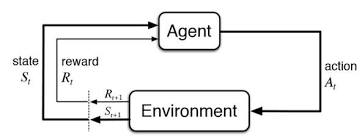
\includegraphics[width=0.7\textwidth]{img/RL.png}
    \caption{Mô hình cơ bản của Reinforcement Learning}
    \label{fig:ten_label}
\end{figure}


Một bài toán RL thường bao gồm các thành phần sau:
\begin{itemize}
    \item \textbf{State (S)}: Mô tả trạng thái hiện tại của môi trường.
    \item \textbf{Action (A)}: Tập các hành động mà agent có thể thực hiện.
    \item \textbf{Reward (R)}: Giá trị phản hồi từ môi trường sau khi agent thực hiện hành động.
    \item \textbf{Policy ($\pi$)}: Chiến lược lựa chọn hành động của agent.
    \item \textbf{Episode}: Chuỗi tương tác liên tục từ trạng thái khởi đầu đến trạng thái kết thúc.
\end{itemize}

Bài toán RL thường được mô hình hóa dưới dạng Markov Decision Process (MDP):

\[
MDP = (S, A, P, R, \gamma)
\]

Trong đó:

\begin{itemize}
    \item $S$: tập trạng thái.
    \item $A$: tập hành động.
    \item $P$: xác suất chuyển trạng thái.
    \item $R$: hàm reward.
    \item $\gamma$: hệ số discount factor.
\end{itemize}


\section{Thuật toán Deep Q-Network (DQN)}

Deep Q-Network (DQN) là thuật toán thuộc nhóm Deep Reinforcement Learning, được phát triển nhằm cải thiện Q-Learning trong các môi trường có không gian trạng thái lớn. Thay vì sử dụng bảng Q-Table, DQN sử dụng mạng neural sâu để xấp xỉ hàm giá trị hành động $Q(s,a)$.

Trong Reinforcement Learning, agent tương tác với môi trường thông qua trạng thái $s$, thực hiện hành động $a$, nhận phần thưởng $r$ và chuyển sang trạng thái tiếp theo $s'$. Mục tiêu của agent là tối đa hóa tổng phần thưởng tích lũy:

\[
R_t = \sum_{k=0}^{\infty} \gamma^k r_{t+k+1}
\]

Trong đó:
\begin{itemize}
    \item $R_t$: tổng phần thưởng tích lũy tại thời điểm $t$
    \item $\gamma$: hệ số discount factor $(0 < \gamma < 1)$
    \item $r_{t+k+1}$: phần thưởng trong tương lai
\end{itemize}

DQN sử dụng mạng neural để xấp xỉ hàm giá trị Q:

\[
Q(s,a;\theta)
\]

Trong đó:
\begin{itemize}
    \item $s$: trạng thái hiện tại
    \item $a$: hành động
    \item $\theta$: trọng số của mạng neural
\end{itemize}

Giá trị Q được cập nhật dựa trên phương trình Bellman:

\[
Q(s,a)=r+\gamma \max_{a'}Q(s',a')
\]

Trong đó:
\begin{itemize}
    \item $r$: phần thưởng nhận được
    \item $s'$: trạng thái tiếp theo
    \item $\gamma$: hệ số discount factor
    \item $\max_{a'}Q(s',a')$: giá trị Q lớn nhất tại trạng thái kế tiếp
\end{itemize}

Trong quá trình huấn luyện, DQN tối ưu giá trị dự đoán thông qua target value:

\[
y = r+\gamma \max_{a'}Q(s',a';\theta^{-})
\]

Trong đó:
\begin{itemize}
    \item $y$: giá trị mục tiêu
    \item $\theta^{-}$: trọng số của Target Network
\end{itemize}

Hàm mất mát (Loss Function) của DQN được xác định như sau:

\[
L(\theta)=\mathbb{E}\left[(y-Q(s,a;\theta))^2\right]
\]

Trong đó:
\begin{itemize}
    \item $Q(s,a;\theta)$: giá trị Q dự đoán từ mạng neural
    \item $y$: giá trị mục tiêu
\end{itemize}

Gradient được sử dụng để cập nhật trọng số mạng neural:

\[
\nabla_{\theta}L(\theta)=
\mathbb{E}\left[(y-Q(s,a;\theta))
\nabla_{\theta}Q(s,a;\theta)\right]
\]

Trong đó:
\begin{itemize}
    \item $y$: giá trị mục tiêu (target value)
    \item $Q(s,a;\theta)$: giá trị Q được dự đoán bởi mạng neural
    \item $\nabla_{\theta}Q(s,a;\theta)$: đạo hàm của hàm Q theo trọng số mạng neural
    \item $\theta$: tập trọng số của mạng neural
\end{itemize}

Để cân bằng giữa exploration và exploitation, DQN sử dụng chiến lược $\varepsilon$-greedy:

\[
a=
\begin{cases}
\text{random action}, & \text{with probability } \varepsilon \\
\arg\max_a Q(s,a), & \text{with probability } 1-\varepsilon
\end{cases}
\]



\section{Proximal Policy Optimization (PPO)}

Proximal Policy Optimization (PPO) là một thuật toán thuộc nhóm Policy Gradient trong Reinforcement Learning, được đề xuất bởi OpenAI nhằm cải thiện tính ổn định và hiệu quả trong quá trình huấn luyện policy. PPO được thiết kế để khắc phục các hạn chế của các phương pháp Policy Gradient truyền thống và Trust Region Policy Optimization (TRPO), đặc biệt là hiện tượng cập nhật policy quá lớn dẫn đến mất ổn định hoặc không hội tụ trong quá trình học.

PPO thuộc kiến trúc Actor--Critic, bao gồm hai thành phần chính là Actor và Critic. Actor chịu trách nhiệm học policy để lựa chọn hành động phù hợp với trạng thái hiện tại của môi trường, trong khi Critic có nhiệm vụ ước lượng giá trị của trạng thái thông qua hàm value function. Sự kết hợp giữa hai thành phần này giúp giảm phương sai (variance) của gradient và tăng độ ổn định trong quá trình huấn luyện.

\begin{figure}[!htbp]
\centering
\small
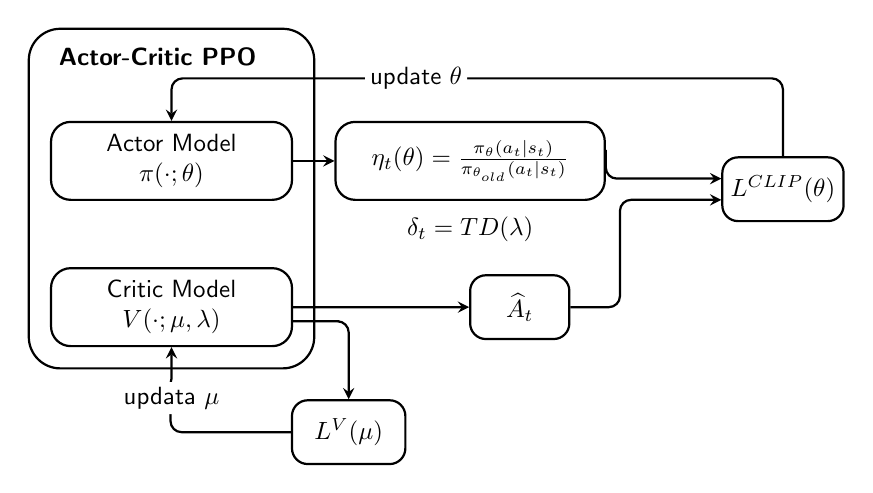
\begin{tikzpicture}[
    scale=0.9, transform shape,
    % Định nghĩa style các khối cố định độ rộng để text không làm phình node
    block/.style={
        draw=black, thick, rounded corners=2.5mm, 
        minimum width=3.4cm, minimum height=1.1cm, 
        align=center, fill=white, font=\sffamily
    },
    small/.style={
        draw=black, thick, rounded corners=2mm, 
        minimum width=1.4cm, minimum height=0.9cm, 
        align=center, fill=white, font=\sffamily
    },
    line/.style={
        ->, >=stealth, thick, rounded corners=4pt
    }
]

    % --- 1. NHÓM ACTOR & CRITIC (Gốc tọa độ) ---
    \node[block] (actor) at (0, 0) {Actor Model\\$\pi(\cdot ; \theta)$};
    % Đẩy Critic xuống dưới Actor cố định 1.5cm
    \node[block] (critic) at ([yshift=-1.5cm]actor.south) {Critic Model\\$V(\cdot ; \mu, \lambda)$};

    % Khung bao Actor-Critic PPO: Dựa hoàn toàn vào góc của actor và critic để không bao giờ bị lệch
    \draw[thick, rounded corners=4mm] 
        ([xshift=-0.3cm, yshift=1.3cm]actor.north west) rectangle ([xshift=0.3cm, yshift=-0.3cm]critic.south east);
    % Nhãn chữ đặt động ở giữa
    \node[font=\sffamily\bfseries, anchor=west] at ([yshift=0.9cm]actor.north west) {Actor-Critic PPO};
    
    % --- 2. CÁC KHỐI TÍNH TOÁN Ở GIỮA (Dịch chuyển theo trục X từ khối bên trái) ---
    % Khối eta_t nằm ngang hàng với Actor, cách sang phải 2.5cm
    \node[block, minimum width=3.8cm] (ratio) at ([xshift=2.5cm]actor.east) {$\eta_t(\theta) = \frac{\pi_\theta(a_t \mid s_t)}{\pi_{\theta_{\text{old}}}(a_t \mid s_t)}$};
    
    % Khối Advantage A_t nằm dịch sang phải từ Critic
    \node[small] (advantage) at ([xshift=3.2cm, yshift=0cm]critic.east) {$\widehat{A}_t$};
    
    % Nhãn delta_t nằm độc lập ngay dưới ratio
    \node (delta) at ([yshift=-0.4cm]ratio.south) [font=\sffamily] {$\delta_t = \text{TD}(\lambda)$};

    % --- 3. CÁC KHỐI LOSS (Nằm ngoài cùng và phía dưới) ---
    % Khối L^CLIP dịch sang phải từ khối ratio
    \node[small, minimum width=1.6cm] (l_clip) at ([xshift=2.5cm, yshift=-0.4cm]ratio.east) {$\text{L}^{\text{CLIP}}(\theta)$};
    
    % Khối L^V nằm ngay dưới khối Critic
    \node[small, minimum width=1.6cm] (l_v) at ([xshift=2.5cm, yshift=-1.2cm]critic.south) {$\text{L}^{\text{V}}(\mu)$};

    % --- 4. HỆ THỐNG ĐƯỜNG NỐI MŨI TÊN ---
    
    % Từ Actor thẳng sang Ratio
    \draw[line] (actor.east) -- (ratio.west);
    
    % Từ Critic sang Khối Advantage
    \draw[line] (critic.east) -- (advantage.west);
    
    % Từ Critic đi xuống thẳng khối L^V
    \draw[line] ([yshift=-0.2cm]critic.east) -- ++(0.5,0) -| (l_v.north);
    
    % Đường gom từ Ratio và Advantage vào L^CLIP
    \draw[line] (ratio.east) -- ++(0,0) |- ([yshift=0.15cm]l_clip.west);
    \draw[line] (advantage.east) -- ++(0.7,0) |- ([yshift=-0.15cm]l_clip.west);
    
    % --- 5. ĐƯỜNG PHẢN HỒI CẬP NHẬT (FEEDBACK LOOPS) ---

    % Update theta: Từ đỉnh L^CLIP vòng lên trên đỉnh Actor
    \draw[line] (l_clip.north) -- ++(0,1.1) -| (actor.north)
        node[pos=0.3, fill=white, inner sep=2pt, font=\sffamily] {update $\theta$};
         
    % Update mu: Từ đáy L^V đi vòng sang trái rồi đâm thẳng vào đáy Critic
    \draw[line] (l_v.west) -- ++(-1.7,0) |- ([yshift=-0.6cm]critic.south) -- (critic.south)
        node[pos=-0.2, fill=white, inner sep=2pt, font=\sffamily] {updata $\mu$};

\end{tikzpicture}
\caption{Sơ đồ hoàn chỉnh kiến trúc Actor-Critic PPO cấu trúc lại}
\label{fig:actor_critic_ppo_perfect}
\end{figure}


Trong Reinforcement Learning, policy là một phân phối xác suất ánh xạ từ trạng thái sang hành động:


\[
\pi(a|s)
\]

Trong đó:
\begin{itemize}
    \item $s$: trạng thái của môi trường
    \item $a$: hành động được lựa chọn
    \item $\pi(a|s)$: xác suất chọn hành động $a$ tại trạng thái $s$
\end{itemize}

Sau mỗi lần tương tác với môi trường, Critic ước lượng giá trị trạng thái nhằm hỗ trợ Actor cập nhật policy theo hướng tối ưu.

Hàm mục tiêu cơ bản của Policy Gradient được định nghĩa:

\[
J(\theta) = \mathbb{E}_{\pi_\theta}[R_t]
\]

Trong đó:
\begin{itemize}
    \item $J(\theta)$: hàm mục tiêu cần tối ưu
    \item $\pi_\theta$: policy với tham số $\theta$
    \item $R_t$: tổng reward tích lũy
\end{itemize}

Gradient của hàm mục tiêu:

\[
\nabla_\theta J(\theta)
= \mathbb{E}_{\pi_\theta}\left[\nabla_\theta \log \pi_\theta(a_t|s_t)\, R_t \right]
\]

Tuy nhiên, Policy Gradient truyền thống có phương sai cao và khó ổn định. Do đó, PPO sử dụng Advantage Function:

\[
A_t = Q(s_t, a_t) - V(s_t)
\]

Trong đó:
\begin{itemize}
    \item $Q(s_t, a_t)$: giá trị hành động
    \item $V(s_t)$: giá trị trạng thái
\end{itemize}

Nếu $A_t > 0$, hành động tốt hơn kỳ vọng.

Ngược lại nếu $A_t < 0$, hành động kém hơn kỳ vọng.

PPO định nghĩa probability ratio giữa policy mới và policy cũ:

\[
r_t(\theta) =
\frac{\pi_\theta(a_t|s_t)}{\pi_{\theta_{\text{old}}}(a_t|s_t)}
\]

Tỷ lệ này phản ánh mức độ thay đổi của policy giữa hai lần cập nhật.

Hàm objective chính của PPO (clipped surrogate objective):

\[
L^{CLIP}(\theta)
=
\mathbb{E}_t \left[
\min \Big(
r_t(\theta) A_t,\;
\text{clip}(r_t(\theta), 1-\epsilon, 1+\epsilon) A_t
\Big)
\right]
\]

Trong đó:
\begin{itemize}
    \item $r_t(\theta)$: probability ratio
    \item $A_t$: advantage estimate
    \item $\epsilon$: clipping parameter
\end{itemize}

Cơ chế clipping giới hạn mức thay đổi của policy trong khoảng $[1-\epsilon, 1+\epsilon]$, giúp tránh cập nhật quá lớn gây mất ổn định hoặc divergence.

Quá trình huấn luyện PPO gồm các bước:

Agent tương tác với môi trường, thu thập trajectory, tính reward và advantage, sau đó tối ưu hàm clipped objective bằng mini-batch gradient descent. Thuật toán thường thực hiện nhiều epoch trên cùng một batch dữ liệu nhằm tăng sample efficiency.

Nhờ cơ chế cập nhật ổn định và hiệu quả trong không gian trạng thái lớn, PPO là một trong những thuật toán Deep Reinforcement Learning được sử dụng phổ biến trong các bài toán điều khiển, quản lý tài nguyên và hệ thống phân tán.


\section{Các nghiên cứu liên quan}

Trong những năm gần đây, việc ứng dụng các mô hình học máy vào vấn đề tự phục hồi của các hệ thống phân tán vẫn đang là chủ đề mới

Trong bài “AI-enhanced self-healing Kubernetes for scalable cloud operations”, tác giả Veeresh Nunavath đã chỉ ra rằng mặc dù Kubernetes sở hữu các tính năng tự phục hồi tích hợp sẵn mạnh mẽ, chúng vẫn chỉ mang tính chất phản ứng và bị giới hạn về phạm vi. Nghiên cứu khẳng định việc tích hợp AI sẽ giúp cơ chế tự phục hồi truyền thống tiến hóa thành các hệ thống tự trị, có khả năng thích nghi và dự đoán lỗi. Tuy nhiên, bài viết chủ yếu dừng lại ở múc độ kiến trúc tổng thể và các chiến lược triển khai lý thuyết.

Nghiên cứu “Self-Healing Infrastructure: Leveraging Reinforcement Learning for Autonomous Cloud Recovery and Enhanced Resilience” đã đề xuất một khung cơ sở hạ tầng tự phục hồi đa tầng kết hợp giữa phân tích dự đoán và Reinforcement Learning (RL). Điểm đáng chú ý trong nghiên cứu này là dùng thuật toán PPO làm bộ não điều phối. Tác nhân PPO liên tục thu thập dữ liệu đo lường như CPU, RAM và network để đưa ra các hành động phục hồi động dựa trên một hàm phần thưởng đánh giá tính khả dụng của hệ thống.

Kế thừa các quan điểm từ hai nghiên cứu trên, đồ tài này sẽ tiếp tục đi sâu vào việc khai thác thuật toán PPO trong môi trường Kubernetes, tập trung thiết kế không gian trạng thái đa chiều và tinh chỉnh hàm phần thưởng nhằm giải quyết cho 5 kịch bản lỗi phổ biến trong kiến trúc microservices.

